\section{The corpus}
\label{sec:corpus}

Release 1.1 (Table~\ref{tab:corpus}, Figure~\ref{fig:corpus}) is one JSON record per conversation: NARA's metadata and subject log, audio sources, withdrawn spans, speaker segments, and every word with its timing, speaker, confidence and source (Parakeet, both recognizers, a Whisper fill, a model edit or a correction by ear). Each edit keeps what it replaced and why. Plain-text transcripts and the raw recognizer outputs ship with it. A browsing application in the repository presents the corpus by day, conversation and person and plays each transcript in sync with the audio; no language model writes its text.

\begin{table}[t]
\centering
\caption{The Nixon Corpus, release 1.1.}
\label{tab:corpus}
\small
\begin{tabularx}{\linewidth}{@{}l X@{}}
\toprule
Conversations & 19,426 (February 16, 1971 -- July 12, 1973), 17,343 with words \\
Audio & 2,206 hours: 6,548 telephone, 6,224 Oval Office, 4,435 EOB, 2,003 Camp David, 216 Cabinet Room \\
Words & 18,994,348, each with start and end time, source and confidence; every model edit marked and reversible \\
Speakers & 63\% of words named; of 1,461 hours of scored speech, 1,023 named (Nixon 637, Haldeman 99, Kissinger 79) \\
Context & NARA date and location for every conversation, participants for all but 35, subject log for 94\% \\
Format & JSON (gzip), plain text, metadata table, raw layers, checksums; 776\,MB \\
\bottomrule
\end{tabularx}
\end{table}

\begin{figure}[t]
  \centering
  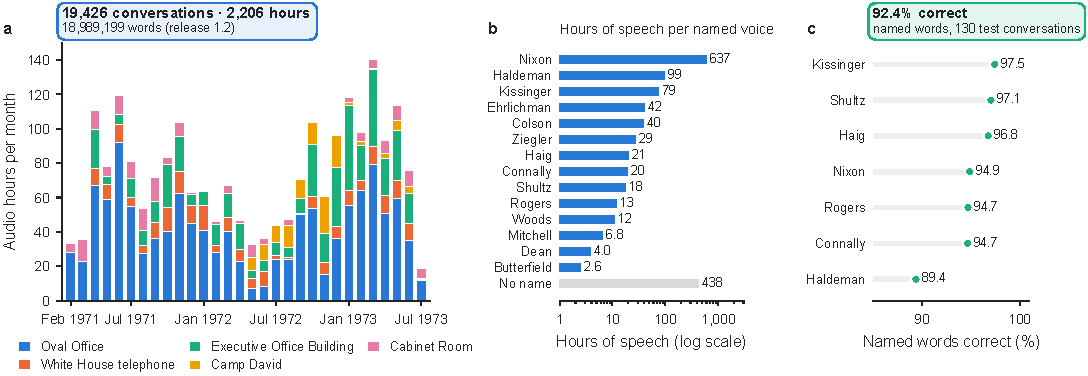
\includegraphics[width=\linewidth]{figures/fig4_corpus.pdf}
  \caption{The corpus. \textbf{a},~Audio hours per month by recording location, February 1971 to July 1973. \textbf{b},~Hours of speech per named voice (segments named at probability 0.7 or more; log scale) and the 438 scored hours without a name. \textbf{c},~Named words correct on the 130 held-out test conversations outside the classifier's training data, for voices with at least 200 named words.}
  \label{fig:corpus}
\end{figure}
